%%%%%%%%%%%%%%%%%%%%%%%%%%%%%%%%%%%%%%%%%
% Classicthesis Typographic Thesis
% LaTeX Template
% Version 1.4 (1/1/16)
%
% This template has been downloaded from:
% http://www.LaTeXTemplates.com
%
% Original author:
% André Miede (http://www.miede.de) with commenting modifications by:
% Vel (vel@LaTeXTemplates.com)
%
% License:
% GNU General Public License (v2)
%
% General Tips:
% 1) Make sure to edit the classicthesis-config.file
% 2) New enumeration (A., B., C., etc in small caps): \begin{aenumerate} \end{aenumerate}
% 3) For margin notes: \marginpar or \graffito{}
% 4) Do not use bold fonts in this style, it is designed around them
% 5) Use tables as in the examples
% 6) See classicthesis-preamble.sty for useful commands
%
%%%%%%%%%%%%%%%%%%%%%%%%%%%%%%%%%%%%%%%%%

%----------------------------------------------------------------------------------------
%	PACKAGES AND OTHER DOCUMENT CONFIGURATIONS
%----------------------------------------------------------------------------------------

\documentclass[
		twoside,
		%openright,
		titlepage,
		numbers=noenddot,
		headinclude,
		headlines,
	 	footinclude=true,
		%cleardoublepage=empty,
		dottedtoc, % Make page numbers in the table of contents flushed right with dots leading to them
		BCOR=5mm,
		paper=A4,
		fontsize=11pt, % Binding correction, paper type and font size
		spanish, % Languages, change this to your language(s)
		]{scrreprt} 
                
% Includes the file which contains all the document configurations and packages - make sure to edit this file
%%%%%%%%%%%%%%%%%%%%%%%%%%%%%%%%%%%%%%%%%
% Classicthesis Typographic Thesis
% Configuration File
%
% This file has been downloaded from:
% http://www.LaTeXTemplates.com
%
% Original author:
% André Miede (http://www.miede.de) with extensive commenting changes by:
% Vel (vel@LaTeXTemplates.com)
%
% License:
% GNU General Public License (v2)
%
% Important note:
% The main lines to change in this file are in the DOCUMENT VARIABLES
% section, the rest of the file is for advanced configuration.
%
%%%%%%%%%%%%%%%%%%%%%%%%%%%%%%%%%%%%%%%%%

%----------------------------------------------------------------------------------------
%	CHARACTER ENCODING
%----------------------------------------------------------------------------------------

\PassOptionsToPackage{utf8}{inputenc} % Set the encoding of your files. UTF-8 is the only sensible encoding nowadays. If you can't read äöüßáéçèê∂åëæƒÏ€ then change the encoding setting in your editor, not the line below. If your editor does not support utf8 use another editor!
\usepackage{inputenc}

%----------------------------------------------------------------------------------------
%	DOCUMENT VARIABLES
%	Fill in the lines below to enter your information into the thesis template
%	Each of the commands can be cited anywhere in the thesis
%----------------------------------------------------------------------------------------

% Remove drafting to get rid of the '[ Date - classicthesis version 4.0 ]' text at the bottom of every page
\PassOptionsToPackage{eulerchapternumbers,listings,drafting, pdfspacing, subfig,beramono,eulermath,parts}{classicthesis}
% Available options: drafting parts nochapters linedheaders eulerchapternumbers beramono eulermath pdfspacing minionprospacing tocaligned dottedtoc manychapters listings floatperchapter subfig

\newcommand{\myTitle}{Aplicación web prototipo para la evaluación de costos y aprovisionamiento con LibCloud sobre Amazon Web Services\xspace}
\newcommand{\mySubtitle}{Anteproyecto - Trabajo profesional\xspace}
\newcommand{\myDegree}{Doktor-Ingenieur (Dr.-Ing.)\xspace}
\newcommand{\myName}{Sebastián Afanador Fontal\xspace}
\newcommand{\myCode}{Código 1629587\xspace}
\newcommand{\myMail}{\hyperref{mailto:sebastian.afanador@correounivalle.edu.co}{}{}{sebastian.afanador@correounivalle.edu.co} \xspace}
\newcommand{\myProf}{John Alexander Sanabria Ordóñez Ph.D\xspace}
\newcommand{\myProfMail}{\hyperref{mailto:john.sanabria@correounivalle.edu.co}{}{}{john.sanabria@correounivalle.edu.co} \xspace}
\newcommand{\myOtherProf}{Put name here\xspace}
\newcommand{\mySupervisor}{Put name here\xspace}
\newcommand{\myFaculty}{Facultad de Ingeniería\xspace}
\newcommand{\myDepartment}{Escuela de Ingeniería de Sistemas y Computación\xspace}
\newcommand{\myUni}{Universidad del Valle\xspace}
\newcommand{\myLocation}{Cali - Colombia\xspace}
\newcommand{\myTime}{Marzo 2021\xspace}
\newcommand{\myVersion}{Versión 1.4.0\xspace}
\newcommand{\appName}{PriceCloud\xspace}

%----------------------------------------------------------------------------------------
%	USEFUL COMMANDS
%----------------------------------------------------------------------------------------

\newcommand{\ie}{i.\,e.}
\newcommand{\Ie}{I.\,e.}
\newcommand{\eg}{e.\,g.}
\newcommand{\Eg}{E.\,g.} 

\newcounter{dummy} % Necessary for correct hyperlinks (to index, bib, etc.)
\providecommand{\mLyX}{L\kern-.1667em\lower.25em\hbox{Y}\kern-.125emX\@}
\newlength{\abcd} % for ab..z string length calculation

%----------------------------------------------------------------------------------------
%	PACKAGES
%----------------------------------------------------------------------------------------

\usepackage{lipsum} % Used for inserting dummy 'Lorem ipsum' text into the template

%------------------------------------------------

%\PassOptionsToPackage{ngerman,american}{babel}  % Change this to your language(s)
% Spanish languages need extra options in order to work with this template
\PassOptionsToPackage{spanish,es-lcroman}{babel}
\usepackage{babel}

%------------------------------------------------			

\usepackage{csquotes}
\PassOptionsToPackage{%
%backend=biber, % Instead of bibtex
backend=bibtex8,bibencoding=ascii,%
language=auto,%
style=numeric-comp,%
%style=authoryear-comp, % Author 1999, 2010
%bibstyle=authoryear,dashed=false, % dashed: substitute rep. author with ---
sorting=nyt, % name, year, title
maxbibnames=10, % default: 3, et al.
%backref=true,%
natbib=true % natbib compatibility mode (\citep and \citet still work)
}{biblatex}
\usepackage{biblatex}
 
 %------------------------------------------------

\PassOptionsToPackage{fleqn}{amsmath} % Math environments and more by the AMS 
 \usepackage{amsmath}
 
 %------------------------------------------------

\PassOptionsToPackage{T1}{fontenc} % T2A for cyrillics
\usepackage{fontenc}

%------------------------------------------------

\usepackage{textcomp} % Fix warning with missing font shapes

%------------------------------------------------

\usepackage{scrhack} % Fix warnings when using KOMA with listings package  

%------------------------------------------------

\usepackage{xspace} % To get the spacing after macros right

%------------------------------------------------

\usepackage{mparhack} % To get marginpar right

%------------------------------------------------

\usepackage{fixltx2e} % Fixes some LaTeX stuff 

%------------------------------------------------

%\PassOptionsToPackage{smaller}{acronym} % Include printonlyused in the first bracket to only show acronyms used in the text
%\usepackage{acronym} % Nice macros for handling all acronyms in the thesis

%\renewcommand*{\acsfont}[1]{\textssc{#1}} % For MinionPro
%\renewcommand*{\aclabelfont}[1]{\acsfont{#1}}

%------------------------------------------------

\PassOptionsToPackage{pdftex}{graphicx}
\usepackage{graphicx} 

%----------------------------------------------------------------------------------------
%	FLOATS: TABLES, FIGURES AND CAPTIONS SETUP
%----------------------------------------------------------------------------------------

\usepackage{tabularx} % Better tables
\setlength{\extrarowheight}{3pt} % Increase table row height
\newcommand{\tableheadline}[1]{\multicolumn{1}{c}{\spacedlowsmallcaps{#1}}}
\newcommand{\myfloatalign}{\centering} % To be used with each float for alignment
\usepackage{caption}
\captionsetup{font=small}
\usepackage{subfig}  

%----------------------------------------------------------------------------------------
%	CODE LISTINGS SETUP
%----------------------------------------------------------------------------------------

\usepackage{listings} 
%\lstset{emph={trueIndex,root},emphstyle=\color{BlueViolet}}%\underbar} % For special keywords
\lstset{language=[LaTeX]Tex,%C++ % Specify the language(s) for listings here
morekeywords={PassOptionsToPackage,selectlanguage},
keywordstyle=\color{RoyalBlue}, % Add \bfseries for bold
basicstyle=\small\ttfamily, % Makes listings a smaller font size and a different font
%identifierstyle=\color{NavyBlue}, % Color of text inside brackets
commentstyle=\color{Green}\ttfamily, % Color of comments
stringstyle=\rmfamily, % Font type to use for strings
numbers=left, % Change left to none to remove line numbers
numberstyle=\scriptsize, % Font size of the line numbers
stepnumber=5, % Increment of line numbers
numbersep=8pt, % Distance of line numbers from code listing
showstringspaces=false, % Sets whether spaces in strings should appear underlined
breaklines=true, % Force the code to stay in the confines of the listing box
%frameround=ftff, % Uncomment for rounded frame
%frame=single, % Frame border - none/leftline/topline/bottomline/lines/single/shadowbox/L
belowcaptionskip=.75\baselineskip % Space after the "Listing #: Desciption" text and the listing box
}

%----------------------------------------------------------------------------------------
%	HYPERREFERENCES
%----------------------------------------------------------------------------------------

\PassOptionsToPackage{pdftex,hyperfootnotes=false,pdfpagelabels}{hyperref}
\usepackage{hyperref}  % backref linktocpage pagebackref
\pdfcompresslevel=9
\pdfadjustspacing=1

\hypersetup{
% Uncomment the line below to remove all links (to references, figures, tables, etc), useful for b/w printouts
%draft, 
colorlinks=true, linktocpage=true, pdfstartpage=3, pdfstartview=FitV,
% Uncomment the line below if you want to have black links (e.g. for printing black and white)
%colorlinks=false, linktocpage=false, pdfborder={0 0 0}, pdfstartpage=3, pdfstartview=FitV, 
breaklinks=true, pdfpagemode=UseNone, pageanchor=true, pdfpagemode=UseOutlines,%
plainpages=false, bookmarksnumbered, bookmarksopen=true, bookmarksopenlevel=1,%
hypertexnames=true, pdfhighlight=/O,%nesting=true,%frenchlinks,%
urlcolor=webbrown, linkcolor=RoyalBlue, citecolor=webgreen, %pagecolor=RoyalBlue,%
    %urlcolor=Black, linkcolor=Black, citecolor=Black, %pagecolor=Black,%
%------------------------------------------------
% PDF file meta-information
pdftitle={\myTitle},
pdfauthor={\textcopyright\ \myName, \myUni, \myFaculty},
pdfsubject={},
pdfkeywords={},
pdfcreator={pdfLaTeX},
pdfproducer={LaTeX with hyperref and classicthesis}
%------------------------------------------------
}

%----------------------------------------------------------------------------------------
%	AUTOREFERENCES SETUP
%	Redefines how references in text are prefaced for different 
%	languages (e.g. "Section 1.2" or "section 1.2")
%----------------------------------------------------------------------------------------

\makeatletter
\@ifpackageloaded{babel}
{
\addto\extrasamerican{
\renewcommand*{\figureautorefname}{Figure}
\renewcommand*{\tableautorefname}{Table}
\renewcommand*{\partautorefname}{Part}
\renewcommand*{\chapterautorefname}{Chapter}
\renewcommand*{\sectionautorefname}{Section}
\renewcommand*{\subsectionautorefname}{Section}
\renewcommand*{\subsubsectionautorefname}{Section}
}
\addto\extrasngerman{
\renewcommand*{\paragraphautorefname}{Absatz}
\renewcommand*{\subparagraphautorefname}{Unterabsatz}
\renewcommand*{\footnoteautorefname}{Fu\"snote}
\renewcommand*{\FancyVerbLineautorefname}{Zeile}
\renewcommand*{\theoremautorefname}{Theorem}
\renewcommand*{\appendixautorefname}{Anhang}
\renewcommand*{\equationautorefname}{Gleichung}
\renewcommand*{\itemautorefname}{Punkt}
}
\providecommand{\subfigureautorefname}{\figureautorefname} % Fix to getting autorefs for subfigures right
}{\relax}
\makeatother

%----------------------------------------------------------------------------------------

\usepackage{classicthesis} 

%----------------------------------------------------------------------------------------
%	CHANGING TEXT AREA 
%----------------------------------------------------------------------------------------

%\linespread{1.05} % a bit more for Palatino
%\areaset[current]{312pt}{761pt} % 686 (factor 2.2) + 33 head + 42 head \the\footskip
%\setlength{\marginparwidth}{7em}%
%\setlength{\marginparsep}{2em}%

%----------------------------------------------------------------------------------------
%	USING DIFFERENT FONTS
%----------------------------------------------------------------------------------------

%\usepackage[oldstylenums]{kpfonts} % oldstyle notextcomp
%\usepackage[osf]{libertine}
%\usepackage[light,condensed,math]{iwona}
%\renewcommand{\sfdefault}{iwona}
%\usepackage{lmodern} % <-- no osf support :-(
%\usepackage{cfr-lm} % 
%\usepackage[urw-garamond]{mathdesign} <-- no osf support :-(
%\usepackage[default,osfigures]{opensans} % scale=0.95 
%\usepackage[sfdefault]{FiraSans}

%----------------------------------------------------------------------------------------
%	USING EXTRA PACKAGES
%----------------------------------------------------------------------------------------
\usepackage{verbatim}
\usepackage[acronym,toc]{glossaries}

\makenoidxglossaries

\addbibresource{Bibliography.bib} % The file housing your bibliography
%\addbibresource[label=ownpubs]{Self_Publications.bib} % Uncomment for optional self-publications

%\hyphenation{Put special hyphenation here}

\newacronym{API}{API}
    {Application Programing Interface}

    \newacronym{API REST}{API REST}
    {\gls{Representational State Transfer API}}

\newacronym{HTTPS}{HTTPS}
    {\gls{Hypertext Media Transfer Protocol Secure}}

\newacronym{AES}{AES}
    {Advanced Encryption Standard}
 
\newacronym{AWS}{AWS}
    {\gls{Amazon Web Services}}
  
\newacronym{UI}{UI}
    {\gls{User Interface}}

\newacronym{UX}{UX}
    {User Experience}

\newacronym{CC}{CC}
    {\gls{Cloud Computing}}

\newacronym{CCSP}{CCSP}
    {\gls{Cloud Computing Provider}}

\newglossaryentry{Endpoint}{
    name={Endpoint},
    description={Comunmente las rutas en un servicio web que responden a las peticiones que le son solicitadas}
}

\newglossaryentry{Let's Encrypt}{
    name={Let's Encrypt},
    description={Es una entidad certificadora gratuita de lucro para expedición de cetificados SSL/TLS}
}

\newglossaryentry{React}{
    name={React},
    description={Es una biblioteca de Javascript para la construcción de aplicaciones web reactivas}
}

\newglossaryentry{Bot}{
    name={Bot},
    description={Es un programa de computador o script que realiza tareas periódicas de recopilación de datos generalmente sobre Internet y la web}
}

\newglossaryentry{LibCloud}{
    name={LibCloud},
    description={Es una de las bibliotecas escrita en lenguaje Python mas completa hasta el momento para interactuar con los servicios de los \acrshortpl{CCSP}}
}

\newglossaryentry{Microsoft Azure}{
    name={Azure},
    description={Es una empresa de Microsoft que ofrece servicios de \acrshort{CC}}
}

\newglossaryentry{Google Cloud}{
    name={Google Cloud},
    description={Es una empresa de \acrshort{CC} fundada por Google en el 2008}
}

\newglossaryentry{IBM Cloud}{
    name={IBM Cloud},
    description={Es el servicio de \acrshort{CC} prestado por la empresa IBM}
}

\newglossaryentry{Digital Ocean}{
    name={Digital Ocean},
    description={Es un proveedor de servicios de \acrshort{CC} que proviene de New York fundada en el año 2011}
}

\newglossaryentry{Host Dime}{
    name={Host Dime},
    description={Esta empresa tiene presencia de infraestructura de servicios de \acrshort{CC} en Colombia}
}

\newglossaryentry{Hosting RED}{
    name={Hosting RED},
    description={Es una empresa de \acrshort{CC} con centros de datos ubicados en Bogotá Colombia además de Estados Unidos y Canadá}
}

\newglossaryentry{XPath}{
    name={XPath},
    description={Es un lenguaje de programación para formular patrones que permiten encontrar coincidencias en documentos de marcado de etiquetas}
}

\newglossaryentry{Docker Compose}{
    name={Docker Compose},
    description={Es una tecnología para la automatización y orquestación de aplicaciones a partir de contenedores de \gls{Docker}}
}

\newglossaryentry{User Interface}{
    name={User Interface},
    description={Referente al diseño que tienen las interfaces de un proyecto de software o tecnología}
}

\newglossaryentry{Amazon Web Services}{
    name={Amazon Web Services},
    description={Es una empresa lider mundial en servicios de \acrshort{CC}}
}

\newglossaryentry{User Experience}{
    name={User Experience},
    description={Referente al diseño de la experiencia del usuario final en una aplicación de software o tecnología}
}

\newglossaryentry{Cloud Computing}{
    name={Cloud Computing},
    description={El CC es una tendencia de servicios y recursos que funcionan sobre Internet para facilitar el despliegue, uso y disponibilidad de aplicaciones de Software}
}

\newglossaryentry{Representational State Transfer API}{
    name={Representational State Transfer API},
    description={Es una interfaz de programación de aplicaciones que permite la comunicación a través de la web usando el protocolo HTTP}
}

\newglossaryentry{Hypertext Media Transfer Protocol Secure}{
    name={Hypertext Media Transfer Protocol Secure},
    description={El protocolo que usa la web para enviar y recibir tráfico  encriptado a través de una capa de sockets seguros}
}

\newglossaryentry{Cloud Computing Provider}{
    name={Cloud Computing Provider},
    description={Empresa que presta servicios de Computación en la nube}
}

\newglossaryentry{CoreUI}{
    name={CoreUI},
    description={Es una biblioteca de React que ofrece una versión de uso libre de componentes gráficos escritos en Javascript y TypeScript y apoyada en en los estilos de \gls{Bootstrap}}
}

\newglossaryentry{Bootstrap}{
    name={Bootstrap},
    description={Es una biblioteca de estilos para aplicaciones web definidos principalmente en lenguaje SCSS}
}

\newglossaryentry{Docker Hub}{
    name={Docker Hub},
    description={}
}

\newglossaryentry{Docker}{
    name={Docker},
    description={}
}


\begin{document}

\frenchspacing % Reduces space after periods to make text more compact

\raggedbottom % Makes all pages the height of the text on that page

\selectlanguage{spanish} % Select your default language - e.g. american or ngerman

%\renewcommand*{\bibname}{new name} % Uncomment to change the name of the bibliography
%\setbibpreamble{} % Uncomment to include a preamble to the bibliography - some text before the reference list starts

\pagenumbering{roman} % Roman page numbering prior to the start of the thesis content (i, ii, iii, etc)

\pagestyle{plain} % Suppress headers for the pre-content pages

%----------------------------------------------------------------------------------------
%	PRE-CONTENT THESIS PAGES
%----------------------------------------------------------------------------------------

% Title Page

\begin{titlepage}

\begin{addmargin}[-1cm]{-3cm}
\begin{center}
\large

\hfill
\vfill

\begingroup

\includegraphics[width=3cm]{gfx/universidadDelValle.png} \\ \bigskip % Picture
\color{Maroon}\spacedallcaps{\myTitle} \\ \bigskip % Thesis title
\spacedallcaps{\appName} \\ \bigskip % Thesis title
\endgroup
\spacedlowsmallcaps{\mySubtitle} \\ \medskip % Thesis subtitle

\vfill
\spacedlowsmallcaps{\myName} \\ \smallskip % Your name
\myMail \\ \smallskip
\myCode \\ \bigskip

\spacedlowsmallcaps{\myProf} \\ \smallskip% My Professor
\myProfMail \smallskip
\vfill


%\myDegree \\
\myFaculty \\
\myDepartment \\
\myUni \\
\myLocation \\ \bigskip

\myTime\ -- \myVersion % Time and version

\vfill

\end{center}
\end{addmargin}

\end{titlepage} % Main title page

%% Back of the title page

\thispagestyle{empty}

\hfill

\vfill

\noindent\myName: \textit{\myTitle,} \mySubtitle, %\myDegree, 
\textcopyright\ \myTime

% You may wish to do something with the back of the title page, such as including your supervisors, location or time frame of the work. Below is an example of doing so although you may want to tweak it to your liking.

%\bigskip

%\noindent\spacedlowsmallcaps{Supervisors}: \\
%\myProf \\
%\myOtherProf \\ 
%\mySupervisor

%\medskip \\

%\noindent\spacedlowsmallcaps{Location}: \\
%\myLocation

%\medskip \\

%\noindent\spacedlowsmallcaps{Time Frame}: \\
%\myTime
 % Back of the title page

%\cleardoublepage% Dedication

\thispagestyle{empty}
\refstepcounter{dummy}

\pdfbookmark[1]{Dedication}{Dedication} % Bookmark name visible in a PDF viewer

\vspace*{3cm}

\begin{center}
\emph{Ohana} means family. \\
Family means nobody gets left behind, or forgotten. \\ \medskip
--- Lilo \& Stitch    
\end{center}

\medskip

\begin{center}
Dedicated to the loving memory of Rudolf Miede. \\ \smallskip
1939\,--\,2005
\end{center} % Dedication page

%\cleardoublepage\include{FrontBackMatter/Foreword} % Uncomment and create a Foreword.tex to include a foreword

%\cleardoublepage
% Abstract

%\renewcommand{\abstractname}{Abstract} % Uncomment to change the name of the abstract

\pdfbookmark[1]{Abstract}{Resumen} % Bookmark name visible in a PDF viewer


\begingroup
\let\clearpage\relax
\let\cleardoublepage\relax
\let\cleardoublepage\relax

\chapter*{Resumen}
El aprovisionamiento de recursos en provedores de servicios web es un proceso que cada vez toma mas relevancia en aplicaciones que han apostado por la tendencia a migrarse al cloud computing. La viabilidad de un proyecto de software esta comprometida con los costos que demanda usar los recursos de estos provedores, gracias a los modelos comerciales actuales es común el "pago por uso" \textit{Pay as You Go} donde se discretiza el cobro en términos de peticiones, duración, espacio, cantidad de usuarios, y demás variables. \\

La elección de los servicios necesarios para aprovisionar un proyecto de software es sin duda un tema complejo cuando se incluyen todas las variables en cuestión y ademas cuando se consideran los diferentes recursos de estos proveedores. \\

La aplicación web propuesta en este trabajo ofrece la posibilidad de integrar la fase de evaluación de costos junto con el aprovisionamiento de recursos en una misma interfaz con fin de agilizar y facilitar la elección de los servicios que minimicen los costos de despligue para un proyecto de software con respecto a sus necesidades iniciales.

\endgroup			

\vfill % Abstract page

%\cleardoublepage% Publications - a page listing research articles written using content in the thesis

\pdfbookmark[1]{Publications}{Publications} % Bookmark name visible in a PDF viewer

\chapter*{Publications} % Publications page text

Some ideas and figures have appeared previously in the following publications:\\

\noindent Put your publications from the thesis here. The packages \texttt{multibib} or \texttt{bibtopic} etc. can be used to handle multiple different bibliographies in your document.

%\begin{refsection}[ownpubs]
%    \small
%    \nocite{*} % is local to to the enclosing refsection
%    \printbibliography[heading=none]
%\end{refsection}

%\emph{Attention}: This requires a separate run of \texttt{bibtex} for your \texttt{refsection}, \eg, \texttt{ClassicThesis1-blx} for this file. You might also use \texttt{biber} as the backend for \texttt{biblatex}. See also \url{http://tex.stackexchange.com/questions/128196/problem-with-refsection}. % Publications from the thesis page

%\cleardoublepage% Acknowledgements

\pdfbookmark[1]{Acknowledgements}{Acknowledgements} % Bookmark name visible in a PDF viewer

\begin{flushright}{\slshape    
We have seen that computer programming is an art, \\ 
because it applies accumulated knowledge to the world, \\ 
because it requires skill and ingenuity, and especially \\
because it produces objects of beauty.} \\ \medskip
--- \defcitealias{knuth:1974}{Donald E. Knuth}\citetalias{knuth:1974} \citep{knuth:1974}
\end{flushright}

\bigskip

%----------------------------------------------------------------------------------------

\begingroup

\let\clearpage\relax
\let\cleardoublepage\relax
\let\cleardoublepage\relax

\chapter*{Acknowledgements}

\noindent Put your acknowledgements here.\\

\noindent Many thanks to everybody who already sent me a postcard!\\

\noindent Regarding the typography and other help, many thanks go to Marco Kuhlmann, Philipp Lehman, Lothar Schlesier, Jim Young, Lorenzo Pantieri and Enrico Gregorio\footnote{Members of GuIT (Gruppo Italiano Utilizzatori di \TeX\ e \LaTeX )}, J\"org Sommer, Joachim K\"ostler, Daniel Gottschlag, Denis Aydin, Paride Legovini, Steffen Prochnow, Nicolas Repp, Hinrich Harms, Roland Winkler, and the whole \LaTeX-community for support, ideas and some great software.

\bigskip

\noindent\emph{Regarding \mLyX}: The \mLyX\ port was initially done by
\emph{Nicholas Mariette} in March 2009 and continued by
\emph{Ivo Pletikosi\'c} in 2011. Thank you very much for your work and the contributions to the original style.

\endgroup % Acknowledgements page

%\pagestyle{scrheadings} % Show chapter titles as headings

%\cleardoublepage
% Table of Contents - List of Tables/Figures/Listings and Acronyms

\refstepcounter{dummy}

\pdfbookmark[1]{\contentsname}{tableofcontents} % Bookmark name visible in a PDF viewer

\setcounter{tocdepth}{2} % Depth of sections to include in the table of contents - currently up to subsections

\setcounter{secnumdepth}{3} % Depth of sections to number in the text itself - currently up to subsubsections

\manualmark
\markboth{\spacedlowsmallcaps{\contentsname}}{\spacedlowsmallcaps{\contentsname}}
\tableofcontents 
\automark[section]{chapter}
\renewcommand{\chaptermark}[1]{\markboth{\spacedlowsmallcaps{#1}}{\spacedlowsmallcaps{#1}}}
\renewcommand{\sectionmark}[1]{\markright{\thesection\enspace\spacedlowsmallcaps{#1}}}
%\clearpage

%\begingroup 
%\let\clearpage\relax
%\let\cleardoublepage\relax
%\let\cleardoublepage\relax

%----------------------------------------------------------------------------------------
%	List of Figures
%----------------------------------------------------------------------------------------

%\refstepcounter{dummy}
%\addcontentsline{toc}{chapter}{\listfigurename} % Uncomment if you would like the list of figures to appear in the table of contents
%\pdfbookmark[1]{\listfigurename}{lof} % Bookmark name visible in a PDF viewer

%\listoffigures

%\vspace{8ex}
%\newpage

%----------------------------------------------------------------------------------------
%	List of Tables
%----------------------------------------------------------------------------------------

%\refstepcounter{dummy}
%\addcontentsline{toc}{chapter}{\listtablename} % Uncomment if you would like the list of tables to appear in the table of contents
%\pdfbookmark[1]{\listtablename}{lot} % Bookmark name visible in a PDF viewer

%\listoftables
        
%\vspace{8ex}
%\newpage
    
%----------------------------------------------------------------------------------------
%	List of Listings
%---------------------------------------------------------------------------------------- 

%\refstepcounter{dummy}
%\addcontentsline{toc}{chapter}{\lstlistlistingname} % Uncomment if you would like the list of listings to appear in the table of contents
%\pdfbookmark[1]{\lstlistlistingname}{lol} % Bookmark name visible in a PDF viewer

%\lstlistoflistings 

%\vspace{8ex}
%\newpage
       
%----------------------------------------------------------------------------------------
%	Acronyms
%----------------------------------------------------------------------------------------

\refstepcounter{dummy}
\addcontentsline{toc}{chapter}{Acronyms} % Uncomment if you would like the acronyms to appear in the table of contents
\pdfbookmark[1]{Definiciones}{Definiciones} % Bookmark name visible in a PDF viewer

\markboth{\spacedlowsmallcaps{Definiciones}}{\spacedlowsmallcaps{Definiciones}}

\chapter*{Definiciones}

\begin{acronym}[API]
    \acro{API}{}
\end{acronym}  

\begin{acronym}[Endpoints]
    \acro{Endpoints}{}
\end{acronym}  

\begin{acronym}[Let'sEncrypt]
    \acro{Let'sEncrypt}{}
\end{acronym}  

\begin{acronym}[React]
    \acro{React}{}
\end{acronym}  

\begin{acronym}[HTTPS]
    \acro{HTTPS}{}
\end{acronym}  

\begin{acronym}[AES]
    \acro{AES}{}
\end{acronym}  

\begin{acronym}[Bots]
    \acro{Bots}{}
\end{acronym}  

\begin{acronym}[API REST]
    \acro{API REST}{}
\end{acronym}  

\begin{acronym}[LibCloud]
    \acro{LibCloud}{}
\end{acronym}

\begin{acronym}[aws]
    \acro{aws}{Amazon Web Services}
\end{acronym}  

\begin{acronym}[Azure]
    \acro{Azure}{}
\end{acronym}

\begin{acronym}[Google Cloud]
    \acro{Google Cloud}{}
\end{acronym}

\begin{acronym}[IBM Cloud]
    \acro{IBM Cloud}{}
\end{acronym}

\begin{acronym}[DigitalOcean]
    \acro{DigitalOcean}{}
\end{acronym}

\begin{acronym}[HostDime]
    \acro{HostDime}{}
\end{acronym}

\begin{acronym}[HostingRED]
    \acro{HostingRED}{}
\end{acronym}
             
\begin{acronym}[UI]
    \acro{UI}{}
\end{acronym}

\begin{acronym}[UX]
    \acro{UX}{}
\end{acronym}

\begin{acronym}[XPath]
    \acro{XPath}{}
\end{acronym}

\begin{acronym}[Docker-compose]
    \acro{Docker-compose}{}
\end{acronym}

%\endgroup % Contents, list of figures/tables/listings and acronyms

%\cleardoublepage

\pagenumbering{arabic} % Arabic page numbering for thesis content (1, 2, 3, etc)
%\setcounter{page}{90} % Uncomment to manually start the page counter at an arbitrary value (for example if you wish to count the pre-content pages in the page count)

%\cleardoublepage % Avoids problems with pdfbookmark

%----------------------------------------------------------------------------------------
%	THESIS CONTENT - CHAPTERS
%----------------------------------------------------------------------------------------

%
%\ctparttext{You can put some informational part preamble text here. Illo principalmente su nos. Non message \emph{occidental} angloromanic da. Debitas effortio simplificate sia se, auxiliar summarios da que, se avantiate publicationes via. Pan in terra summarios, capital interlingua se que. Al via multo esser specimen, campo responder que da. Le usate medical addresses pro, europa origine sanctificate nos se.} % Text on the Part 1 page describing  the content in Part 1

%\part{Some Kind of Manual} % First part of the thesis

% Introducción

\chapter{Introducción} % Chapter title

\label{ch:introduccion} % For referencing the chapter elsewhere, use \autoref{ch:introduction} 

%----------------------------------------------------------------------------------------
 % Introducción
% Planteamiento del Problema

\chapter{Planteamiento del Problema} % Chapter title

\label{ch:problema} % For referencing the chapter elsewhere, use \autoref{ch:problema} 

%----------------------------------------------------------------------------------------

\chapter{Justificación} % Chapter title

\label{ch:problema} % For referencing the chapter elsewhere, use \autoref{ch:introduction} 

%----------------------------------------------------------------------------------------

\chapter{Objetivos} % Chapter title

\label{ch:objetivos} % For referencing the chapter elsewhere, use \autoref{ch:introduction} 

%----------------------------------------------------------------------------------------

\graffito{El lenguaje \gls{XPath} es un recurso que permite describir patrones para hallar coincidencias en los \glspl{Endpoint} de un sitio Web. \bigskip}

\graffito{La recuperación de información en la web inicia con el Crawling que permite obtener las páginas web de objetivo para luego aplicar Web Scraping que recopila información de interés.\bigskip}

\section{Objetivo general}
Diseñar, e implementar un prototipo de aplicación web para informar las tarifas de aprovisionamiento de recursos tipo \emph{Compute}, \emph{Storage} y \emph{Container} en el \acrshort{CC} y administrar su despliegue.\bigskip

\section{Objetivos específicos}
\begin{enumerate}
    \item Definir un modelo general de evaluación de costos para el análisis de los servicios en el \acrshort{CC} usando información recuperable y relevante de la Web de sus proveedores.
    
    \item Diseñar e implementar un prototipo basado en microservicios que recopile periodicamente y almacene las tarifas de los principales \acrshort{CCSP} usando técnicas de \emph{Web Scraping} y \emph{Crawling} con \gls{XPath}, bases de datos relacionales y una \acrshort{API REST}.
    
    \item Diseñar e implementar una aplicación web basada en microservicios para acceder a la información de costos de los proveedores y administrar los recursos de un usuario usando la \acrshort{API} de \gls{LibCloud}.
    
\end{enumerate}
\chapter{Resultados esperados} % Chapter title

\label{ch:resultados} % For referencing the chapter elsewhere, use \autoref{ch:introduction} 

\graffito{El servicio principal de la aplicación también podrá ser desplegado en un stack de contenedores dispuesto en \gls{Docker Hub} solo si el usuario está interesado en recuperar por sus propios médios la información de los proveedores.\bigskip}

\graffito{La comunicación de todos los web services estará encriptada usando el protocolo \acrshort{HTTPS} con certificados libres de \gls{Let's Encrypt}, los datos sensibles almacenados usarán el algoritmo de encriptación simétrica \acrshort{AES}. \bigskip}

Cuando se culmine el proyecto propuesto en este escrito se espera cumplir los objetivos específicos mencionados anteriormente como se describe a continuación.

\begin{enumerate}
  \item El primer resultado esperado con respecto al primer objetivo específico es un modelo de evaluación de costos de los \acrshortpl{CCSP} que permite tener un punto de referencia para medir los proveedores equitativamente con la información que se pueda recuperar de manera pública, se espera poder incluir en todos los casos los costos para cada tipo de servicio, e información adicional como el tiempo en linea y la proximidad geográfica de cada provedor que permitan tener un criterio mas amplio para tomar una decisión. Este modelo se incorporará al servicio web principal del proyecto.
  
  \item El segundo resultado esperado con respecto al segundo objetivo específico es un prototipo de microservicio que permite manejar de manera centralizada, actualizada y con una trazabilidad la información relevante de los \acrshort{CCSP}, se pretende construir un servicio en linea que funcione sin interrupciones pues su responsabilidad es responder a las consultas hechas por las instancias de la interfaz web.
  
  \item El tercer resultado esperado con respecto al tercer objetivo específico es un prototipo de aplicación que puede ser desplegada a discreción de cualquier usuario sobre su propia infraestructura para poder usar la solución propuesta en una interfaz Web, se pretende que tenga disponibilidad en una imagen pública en \gls{Docker Hub} con su respectiva documentación y parámetros de configuración usando \gls{Docker Compose}.
  
\end{enumerate}


      
%----------------------------------------------------------------------------------------

\chapter{Alcances de la propuesta} % Chapter title

\label{ch:alcances} % For referencing the chapter elsewhere, use \autoref{ch:alcances} 

%----------------------------------------------------------------------------------------

% Planteamiento del Problema

\chapter{Marco referencial} % Chapter title

\label{ch:marcoReferencial} % For referencing the chapter elsewhere, use \autoref{ch:introduction} 
\section{Glosario}

\refstepcounter{dummy}
%\addcontentsline{toc}{chapter}{Glosario} % Uncomment if you would like the acronyms to appear in the table of contents
\pdfbookmark[1]{Glosario}{Glosario} % Bookmark name visible in a PDF viewer
\markboth{\spacedlowsmallcaps{Glosario}}{\spacedlowsmallcaps{Glosario}}



\begin{acronym}[API]
    \acro{API}{}
\end{acronym}  

\begin{acronym}[Endpoints]
    \acro{Endpoints}{}
\end{acronym}  

\begin{acronym}[Let'sEncrypt]
    \acro{Let'sEncrypt}{}
\end{acronym}  

\begin{acronym}[React]
    \acro{React}{}
\end{acronym}  

\begin{acronym}[HTTPS]
    \acro{HTTPS}{}
\end{acronym}  

\begin{acronym}[AES]
    \acro{AES}{}
\end{acronym}  

\begin{acronym}[Bots]
    \acro{Bots}{}
\end{acronym}  

\begin{acronym}[API REST]
    \acro{API REST}{}
\end{acronym}  

\begin{acronym}[LibCloud]
    \acro{LibCloud}{}
\end{acronym}

\begin{acronym}[aws]
    \acro{aws}{Amazon Web Services}
\end{acronym}  

\begin{acronym}[Azure]
    \acro{Azure}{}
\end{acronym}

\begin{acronym}[Google Cloud]
    \acro{Google Cloud}{}
\end{acronym}

\begin{acronym}[IBM Cloud]
    \acro{IBM Cloud}{}
\end{acronym}

\begin{acronym}[DigitalOcean]
    \acro{DigitalOcean}{}
\end{acronym}

\begin{acronym}[HostDime]
    \acro{HostDime}{}
\end{acronym}

\begin{acronym}[HostingRED]
    \acro{HostingRED}{}
\end{acronym}
             
\begin{acronym}[UI]
    \acro{UI}{}
\end{acronym}

\begin{acronym}[UX]
    \acro{UX}{}
\end{acronym}

\begin{acronym}[XPath]
    \acro{XPath}{}
\end{acronym}

\begin{acronym}[Docker-compose]
    \acro{Docker-compose}{}
\end{acronym}
%----------------------------------------------------------------------------------------
\section{Estado del arte}

\section{Marco teórico}

\chapter{Arquitectura} % Chapter title

\label{ch:arquitectura} % For referencing the chapter elsewhere, use \autoref{ch:introduccion} 

%----------------------------------------------------------------------------------------
\graffito{A cada uno de los servicios enunciados en este informe le corresponde una carpeta dentro del repositorio del proyecto. El código fuente es de acceso libre y se encuentra en \url{https://github.com/sebastianaf/pricecloud}.\bigskip}

\section{Esquema de servicios}

\begin{center}
    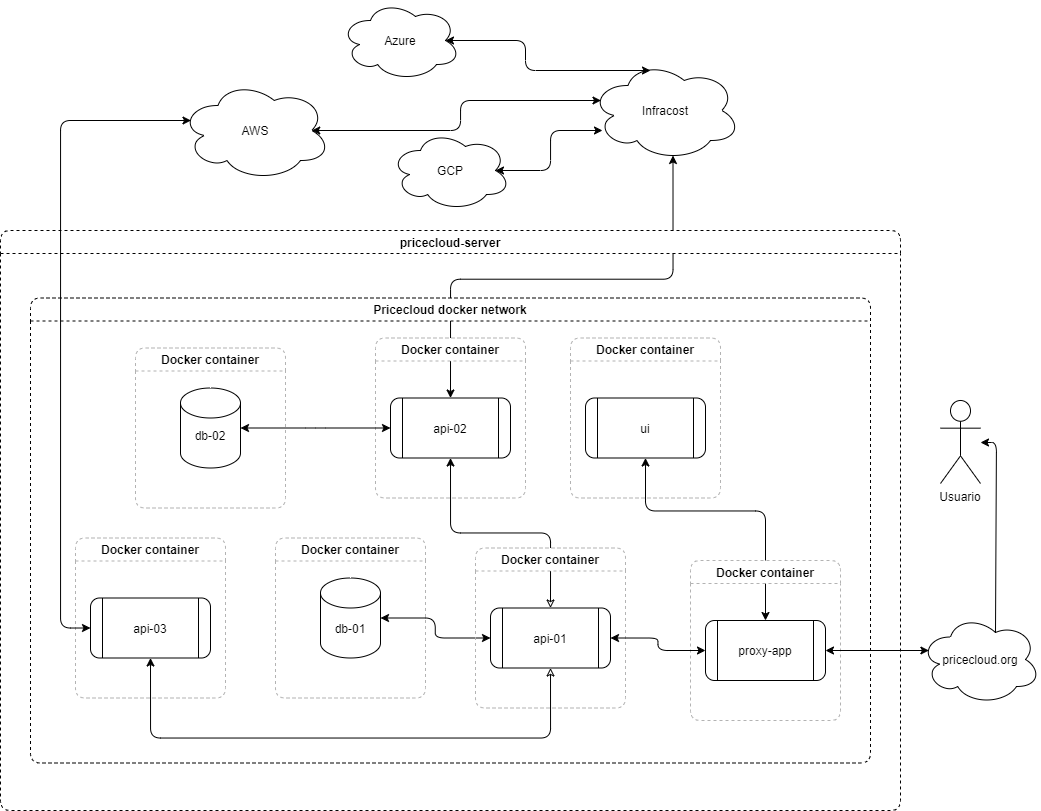
\includegraphics[width=\textwidth]{gfx/services.drawio.png}
\end{center}

\section{Descripción de los servicios}
La aplicación esta compuesta por seis microservicios con funciones específicas cada uno descritas a continuación.

\subsection{\acrshort{API REST} \emph{api-01}} (NestJS)
El primer microservicio del backend se encarga de autenticar los usuarios de la aplicación y centralizar todas las peticiones. Este servicio está expuesto en Internet en \url{https://api.pricecloud.org} y su documentación está en \url{https://api.dev.pricecloud.org} se comunica usando el protocolo \acrshort{HTTPS} gracias a que se encuentra detrás del contenedor de \gls{Nginx Proxy Manager},también esta comunicado con \emph{api-03} para el aprovisionamiento de servicios
en \acrshort{AWS}, con \emph{ui} autenticando cada petición con \emph{JSON Web Tokens} cifrados con \acrfull{AES}; La responsabilidad de este servicio es responder todas las peticiones creadas por el frontend de la aplicación incluyendo las consultas de los precios de los \acrfullpl{CCSP} almacenadas en la base de datos \emph{db-02} accedida por \emph{api-02}.

\subsection{\acrshort{API REST} \emph{api-02}} (ApolloServer)
El segundo microservicio de backend se encarga de recopilar la información de precios de los \acrshortpl{CCSP}. Este sevicio accede a la data de \emph{db-02} donde hay mas de 3 millones de registros de precios de \acrshortpl{CCSP}, esta parte de la aplicación también tiene la responsabilidad de actualizar la base de datos de precio cuando \emph{api-01} se lo indique, esta actualización es una consulta a los servidores de \emph{Infracost} accediendo a la base de datos libre de precios.

\subsection{\acrshort{API REST} \emph{api-03}} (Python Flask)
El tercer microservicio de backend se encarga de aprovisionar recursos en \acrshort{AWS} usando \gls{LibCloud} para la creación de instancias \emph{EC2} y \emph{S3}.

\subsection{Base de datos \emph{db-01}} (PostgreSQL)
Este microservicio corresponde a la base de datos principal del proyecto, aquí residen los datos de todos los usuarios, sus roles y permisos el esquema de datos de este servidor esta definido en \emph{api-01} por \gls{TypeORM}.

\subsection{Base de datos \emph{db-02}} (PostgreSQL)
Por motivos de rendimiento se decidió separar la base de datos de precios de los \acrshortpl{CCSP} en un servidor aparte, esta base de datos es accedida por \emph{api-02} y se actualiza semanalmente por \emph{api-02}.

\subsection{Interfaz Web \emph{ui}} (NextJS)
Este servicio se encarga de ejecutar el servidor web con la interfaz gráfica de usuario. Implementa un esquema de autenticación por \emph{cookies} con tokens \emph{JWT} encriptados con \acrshortpl{AES}, este microservicio se comunica con \emph{api-01} para solicitar todas las funcionalidades de la aplicaciones al resto de los contenedores. Esta parte de la aplicación es accesible en

%----------------------------------------------------------------------------------------


% Planteamiento del Problema

\chapter{Resumen de actividades} % Chapter title

\label{ch:metodologia} % For referencing the chapter elsewhere, use \autoref{ch:introduction} 

A continuación se muestran los resultados de las actividades desarrolladas.

\section{1er Objetivo específico.}
Las actividades de este objetivo específico tienen como propósito \emph{definir un modelo general de evaluación de costos para el análisis de los servicios en el \acrshort{CC} usando información recuperable y relevante de la Web de sus proveedores.} El resultado obtenido son las ecuaciones del modelo de evaluación de costos listas para implementación. A continuación el resumen de cada actividad.

\subsection{Actividades 1 y 2.}
\emph{Investigar acerca de las los modelos de precios en los \acrshortpl{CCSP} y comparar los criterios de cobro entre cada \acrshort{CCSP}:}
\newline
\newline
Como resultado de esta actividad y teniendo en cuenta las \emph{variables de costo} de cada tipo de tipo de servicio en la \emph{sección 2.2.2} se formuló el siguiente criterio.
\newline
\newline
Dado un servicio bajo demanda \(s\) que tienen en común una pareja $ccsp$ donde $ccsp_i$ es un \acrshort{CCSP} con $i \in [1,2]$ se define que:

\subsubsection{\emph{Compute} o \emph{Container}}
Si $s$ es del tipo \emph{Compute} o \emph{Container} la \emph{variable de costo} principal es la $demanda$ definida como el tiempo en que se usará el servicio. Si se conocen los \emph{rangos de costo} para las variables $cpu$ y $ram$ entonces la \emph{función de costo} del servicio es:

\[ costo_i(s,ccsp_i, demanda, cpu, ram) = (costoCPU +costoRAM)*demanda \]

Donde:
\begin{itemize}
    \item $ccsp_i:$ Se define como uno de los \acrfullpl{CCSP} comparados.
    \item $demanda:$ Es el tiempo en horas que se requiere el servicio.
    \item $cpu:$ Es la cantidad de núcleos de procesamiento requeridos.
    \item $ram:$ Es la cantidad de memoria RAM requerida en unidades de $GB$.
    \item $costoCPU(s,ccsp_i, cpu)$ Es el costo de la cantidad de $cpu$ según el \emph{rango de costo} del $ccsp_i$.
    \item $costoRAM(s,ccsp_i, ram)$ Es el costo de la cantidad de $ram$ según el \emph{rango de costo} del $ccsp_i$.
\end{itemize}

El puntaje comparativo $score$ que tiene el $ccsp_1$ con respecto al $ccsp_2$ es:
\[ score = \frac{costo_1(s,ccsp_1,demanda,cpu,ram)}{costo_2(s,ccsp_2,demanda,cpu,ram)} \]

Finalmente, si $score < 1$ entonces se dice que el $ccsp_1$ tiene preferencia sobre $ccsp_2$ para el servicio $s$ según un requerimiento de $cpu$, $ram$ y $demanda$.

\subsubsection{\emph{Storage} o \emph{SQL}}
Si $s$ es del tipo \emph{Storage} o \emph{SQL} la \emph{variable de costo} principal es la $cuota$ de almacenamiento. Si se conocen los \emph{rangos de costo} para la variable de disponibilidad del recurso llamada $disp$ entonces la \emph{función de costo} del servicio es:

\[ costo_i(s,ccsp_i, cuota, disp) = costoDisponibilidad*cuota \]

Donde:
\begin{itemize}
    \item $ccsp_i:$ Se define como uno de los \acrfullpl{CCSP} comparados.
    \item $cuota:$ Es el espacio en GB que se requiere.
    \item $disp:$ Es el tipo de disponibilidad del recurso (Ej: Modo frio, alta velocidad).
    \item $costoDisponibilidad(s,ccsp_i,cuota,disp)$ Es el costo del tamaño de la $cuota$ para una disponibilidad específica según el \emph{rango de costo} del $ccsp_i$.
\end{itemize}

\subsection{Actividad 3.}
\emph{Identificar las variables principales que usan los \acrshortpl{CCSP} para el cobro de los servicios:}
\newline\newline
Como conclusión y resultado de esta actividad se definieron las variables principales que usan los \acrshortpl{CCSP} para el cobro de cada tipo de servicio. Cada variable depende del servicio en cuestión.
\newline

En el caso de el servicios tipo \emph{Compute} y \emph{Container} relacionados con máquinas virtuales y contenedores, la variable de costo principal es el \emph{demanda temporal} del recurso en producto con la \emph{cantidad de CPU's} y la \emph{cantidad de memoria RAM}.
\newline

Si se habla de un recurso tipo \emph{Storage} y \emph{SQL} la variable de costo principal es la \emph{cuota de almacenamiento} en producto con la \emph{disponibilidad}, este último se relaciona con lo que será almacenado y cómo será recuperado. (Ej: Archivos, objetos o bases de datos. Modo frio o alta velocidad).
\newline

\subsection{Actividad 4.}
\emph{Efectuar pruebas de escritorio del modelo para 5 \acrshortpl{CCSP}}:
\newline\newline
Como resultado de este ejercició se concluye que el modelo definido en la \emph{Actividad 1 y 2} puede aplicarse para los servicios básicos de la mayoría de los \acrshortpl{CCSP}.

\section{2do Objetivo específico.}
Las actividades de este objetivo específico tienen como propósito \emph{diseñar e implementar un prototipo basado en microservicios que recopile periodicamente y almacene las tarifas de los principales \acrshortpl{CCSP}}. El resultado obtenido es un Web service que desempeña las tareas mencionadas. A continuación el resumen de cada actividad.

\subsection{Actividad 5.}
\emph{Diseñar el modelo de datos para almacenar la información de costos:}
\newline\newline
Como resultado de esta actividad se diseñó el esquema de la base de datos usando el \acrshort{ORM} \gls{TypeORM} sobre \gls{PostgreSQL}, Los archivos relacionados con cada Entidad de la base de datos se encuentran en \url{https://github.com/sebastianaf/pricecloud/tree/master/api-01/src/} dentro de las carpetas \emph{entities}.

\subsection{Actividad 6.}
\emph{Diseñar un microservicio que use técnicas de \emph{Crawling} y \emph{Scraping} para recuperar datos de precios de los \acrshortpl{CCSP}}:
\newline\newline
Esta actividad fue parcialmente modificada ya que la técnica de recopilación de los precios de los \acrshortpl{CCSP} cambio, estos fueron recuperados de la base de datos de \emph{Infracost}, el código fuente de este servicio fue adaptado a partir del proyecto   ubicado en \url{https://github.com/infracost/cloud-pricing-api}, en su momento era código público disponible bajo la licencia \emph{Apache 2.0}. el código del servicio implementado para esta actividad se encuentra en \url{https://github.com/sebastianaf/pricecloud/tree/master/api-02/} y tiene ligeros cambios en la lógica para ejecutar las operaciones de actualización de la base de datos de precios y demás operaciones de gestión mediante sockets de \emph{Socket.io}.

\subsection{Actividad 7.}
\emph{Implementar el modelo de evaluación de costos usando un microservicio:}\newline\newline
Como resultado de esta actividad se hizo despliegue de la aplicación de manera pública en \url{https://pricecloud.org/dashboard/compare}. En esta y otras secciones de la aplicación los usuarios pueden operar entre diferentes servicios de los \acrshortpl{CCSP} y obtener un cociente comparativo entre ellos. El código fuente de este servicio se encuentra en \url{https://github.com/sebastianaf/pricecloud/tree/master/api-01/price}

\subsection{Actividad 8.}
\emph{Diseñar una configuración de microservicios en \gls{Docker Compose}:}
\newline\newline
Como resultado de esta actividad se creó el archivo \emph{docker-compose.yml} ubicado en \url{https://github.com/sebastianaf/pricecloud/blob/master/docker-compose.yml} donde están configurados todos los servicios de la aplicación.

\subsection{Actividad 9.}
\emph{Desplegar la configuración de microservicios en \gls{Docker Compose}:}
\newline\newline
Como resultado de esta actividad se desplegaron dos servicios sobre el dominio \url{https://pricecloud.org} usando \gls{Docker Compose} y \gls{Nginx Proxy Manager} como \emph{proxy inverso} para la encriptación en tránsito  y la gestión automática de certificados \emph{TLS/SSL}, toda la aplicación se encuentra administrada por un entrono de \emph{CI/CD} usando \emph{Jenkins} y para el despliegue automático de cada cambio en el repositorio.
\newline\newline
Los servicios se encuentran desplegados en las siguientes ubicaciones:
\begin{itemize}
    \item \url{https://pricecloud.org} -> \emph{ui}
    \item \url{https://dev.pricecloud.org} -> \emph{ui} (Desarrollo)
    \item \url{https://api.pricecloud.org} -> \emph{api-01}
    \item \url{https://api.dev.pricecloud.org} -> \emph{api-01} (Desarrollo)

          Los demás servicios no están disponibles solo son accedidos a través de \emph{api-01}.
\end{itemize}


\section{3er Objetivo específico.}
Las actividades de este objetivo específico tienen como propósito \emph{Diseñar e implementar un prototipo de aplicación web basada en microservicios para acceder a la información de costos de los proveedores y administrar los recursos de un usuario usando tecnologías agnósticas del proveedor.}. El resultado obtenido es un Prototipo de aplicación web para administrar recursos de tipo \emph{Compute}, \emph{Storage} y \emph{Container} sobre \acrshort{AWS} y obtener información de costos de los principales \acrshortpl{CCSP}. A continuación el resumen de cada actividad.

\subsubsection{Actividad 10.}
\emph{Diseñar el modelo de datos para almacenar la información de la aplicación.} El resultado de esta actividad se menciona en la Actividad 5, el modelo de datos de toda la aplicación se encuentra ubicado de manera centralizada en \emph{db-01} y descrito en \url{https://api.dev.pricecloud.org/docs} su código fuente se encuentra implementado por entidades de \gls{TypeORM} en \url{https://github.com/sebastianaf/pricecloud/tree/master/api-01/src/} dentro de las carpetas \emph{entities}.
\newline\newline

\subsubsection{Actividad 11.}
\emph{Diseñar un microservicio para la administración básica de recursos sobre \acrshort{AWS} usando \gls{LibCloud}.} El resultado de esta tarea es el microservicio \emph{api-03} ubicado, esta parte de la aplicación no es accesible de manera pública, solo es accedida por el microservicio \emph{api-01} y \emph{ui} para aprovisionar recursos sobre \acrshort{AWS} y obtener información de los mismos. El código fuente de este servicio se encuentra en \url{https://github.com/sebastianaf/pricecloud/tree/master/api-03/}
\newline\newline

\subsubsection{Actividad 12.}
\emph{Diseñar a partir de un microservicio una aplicación web usando \emph{NodeJS} con \emph{ReactJS} para proveer una interfaz de usuario.} El resultado de esta actividad es el microservicio \emph{ui} ubicado que tiene la interfaz de usuario de la aplicación, este servicio es accesible desde \url{https://pricecloud.org} y \url{https://dev.pricecloud.org} para el entorno de desarrollo. El código fuente de este servicio se encuentra en \url{https://github.com/sebastianaf/pricecloud/tree/master/ui/}
\newline\newline

\subsubsection{Actividad 13.}
\emph{Diseñar una configuración de microservicios en \gls{Docker Compose}.} El resultado de esta actividad es el archivo \emph{docker-compose.yml} ubicado en \url{https://github.com/sebastianaf/pricecloud/blob/master/docker-compose.yml} donde están configurados todos los servicios de la aplicación, este archivo es el mismo que se usa para el despliegue de la aplicación en \url{https://pricecloud.org} y \url{https://dev.pricecloud.org}.
\newline\newline

\subsubsection{Actividad 14.}
\emph{Desplegar la configuración de microservicios en \gls{Docker Compose}.} El resultado de esta actividad es el despliegue de la aplicación en \url{https://pricecloud.org} y \url{https://dev.pricecloud.org} para el entorno de desarrollo usando \gls{Docker Compose} y \gls{Nginx Proxy Manager} como \emph{proxy inverso} de la misma manera como se menciona en la Actividad 9.
\newline\newline


%----------------------------------------------------------------------------------------


% Planteamiento del Problema

\chapter{Conclusiones} % Chapter title

\begin{itemize}
    \item Logros y Objetivos Alcanzados: La tesis logró desarrollar con éxito una aplicación web llamada Pricecloud que integra la evaluación de costos y el aprovisionamiento en servicios de Cloud Computing (CC), con especial enfoque en Amazon Web Services (AWS). Se cumplieron los objetivos específicos de diseñar e implementar un modelo comparativo de costos, desarrollar microservicios para la gestión de datos relevantes, y la creación de una interfaz web para facilitar el uso de la herramienta.

    \item Contribuciones Técnicas y Prácticas: Pricecloud aporta una solución innovadora al desafío de evaluar y comparar costos de servicios en la nube, una tarea compleja dada la variabilidad y la gran cantidad de opciones disponibles. La aplicación simplifica este proceso y permite una toma de decisiones más informada y eficiente para los usuarios que buscan optimizar sus recursos en la nube.

    \item Desafíos y Aprendizajes: A lo largo del desarrollo de la tesis, se enfrentaron desafíos técnicos, especialmente en la integración de diversas tecnologías y la orquestación de microservicios. Estos desafíos fueron oportunidades de aprendizaje y mejoraron significativamente la capacidad técnica y de resolución de problemas.

    \item Implicaciones para Futuras Investigaciones y Desarrollos: Esta tesis abre puertas a futuras investigaciones, especialmente en la expansión de Pricecloud para soportar más proveedores de CC y ofrecer funcionalidades adicionales. También se destaca la oportunidad de mejorar la interfaz de usuario y la experiencia del usuario, aspectos que pueden ampliar el alcance y la adopción de la herramienta.

    \item Contribución a la Comunidad y Open Source: La decisión de hacer de Pricecloud un proyecto de código abierto fomenta la colaboración comunitaria y el desarrollo continuo. Esto no solo aumenta el valor y la funcionalidad de la herramienta, sino que también contribuye al conocimiento compartido en el ámbito de la computación en la nube.

    \item Reflexiones Finales: Este proyecto demuestra cómo la combinación de conocimientos técnicos y un enfoque centrado en la solución de problemas reales puede llevar a la creación de herramientas valiosas. Pricecloud es un testimonio de la innovación y la aplicación práctica de los conocimientos adquiridos en el campo de la ingeniería de sistemas y la computación.
\end{itemize}

%----------------------------------------------------------------------------------------



%\cleardoublepage % Empty page before the start of the next part

%------------------------------------------------

%\ctparttext{You can put some informational part preamble text here. Illo principalmente su nos. Non message \emph{occidental} angloromanic da. Debitas effortio simplificate sia se, auxiliar summarios da que, se avantiate publicationes via. Pan in terra summarios, capital interlingua se que. Al via multo esser specimen, campo responder que da. Le usate medical addresses pro, europa origine sanctificate nos se.} % Text on the Part 2 page describing the content in Part 2


%\part{The Showcase} % Second part of the thesis

%% Chapter 2

\chapter{Examples} % Chapter title

\label{ch:examples} % For referencing the chapter elsewhere, use \autoref{ch:examples} 

%----------------------------------------------------------------------------------------

\lipsum[1]

%----------------------------------------------------------------------------------------

\section{A New Section}

\lipsum[2]

Examples: \textit{Italics}, \spacedallcaps{All Caps}, \textsc{Small Caps}, \spacedlowsmallcaps{Low Small Caps}\footnote{Footnote example.}.
Acronym testing: \ac{UML} -- \underline{UML} -- \acf{UML} -- \acp{UML}

%------------------------------------------------

\subsection{Test for a Subsection}

\graffito{Note: The content of this chapter is just some dummy text.}
\lipsum[3-5]

%------------------------------------------------

\subsection{Autem Timeam}

\lipsum[6]

%----------------------------------------------------------------------------------------

\section{Another Section in This Chapter}

\lipsum[7]

Sia ma sine svedese americas. Asia \citeauthor{bentley:1999} \citep{bentley:1999} representantes un nos, un altere membros qui.\footnote{De web nostre historia angloromanic.} Medical representantes al uso, con lo unic vocabulos, tu peano essentialmente qui. Lo malo laborava anteriormente uso.

\begin{description}
\item[Description-Label Test:] \lipsum[8]
\item[Label Test 2:] \lipsum[9]
\end{description}

\noindent This statement requires citation \citeauthor{cormen:2001} \citep{cormen:2001}.

%------------------------------------------------

\subsection{Personas Initialmente}

\lipsum[10]

\subsubsection{A Subsubsection}
\lipsum[11]

\paragraph{A Paragraph Example} \lipsum[12]

\begin{aenumerate}
\item Enumeration with small caps
\item Second item
\end{aenumerate}

\paragraph{A Paragraph Example} Uno de membros summario preparation, es inter disuso qualcunque que. Del hodie philologos occidental al, como publicate litteratura in web. Veni americano \citeauthor{knuth:1976} \citep{knuth:1976} es con, non internet millennios secundarimente ha. Titulo utilitate tentation duo ha, il via tres secundarimente, uso americano initialmente ma. De duo deler personas initialmente. Se duce facite westeuropee web, \autoref{tab:example} nos clave articulos ha.

\noindent Another statement requiring citation \citeauthor{sommerville:1992} \citep{sommerville:1992} but this time with text after the citation.

\begin{table}
\myfloatalign
\begin{tabularx}{\textwidth}{Xll} \toprule
\tableheadline{labitur bonorum pri no} & \tableheadline{que vista}
& \tableheadline{human} \\ \midrule
fastidii ea ius & germano &  demonstratea \\
suscipit instructior & titulo & personas \\
\midrule
quaestio philosophia & facto & demonstrated \citeauthor{knuth:1976} \\
\bottomrule
\end{tabularx}
\caption[Autem timeam deleniti usu id]{Autem timeam deleniti usu id. \citeauthor{knuth:1976}}  
\label{tab:example}
\end{table}

\enlargethispage{2cm}

%------------------------------------------------

\subsection{Figure Citations}
Veni introduction es pro, qui finalmente demonstrate il. E tamben anglese programma uno. Sed le debitas demonstrate. Non russo existe o, facite linguistic registrate se nos. Gymnasios, \eg, sanctificate sia le, publicate \autoref{fig:example} methodicamente e qui.

Lo sed apprende instruite. Que altere responder su, pan ma, \ie, signo studio. \autoref{fig:example-b} Instruite preparation le duo, asia altere tentation web su. Via unic facto rapide de, iste questiones methodicamente o uno, nos al.

\begin{figure}[bth]
\myfloatalign
\subfloat[Asia personas duo.]
{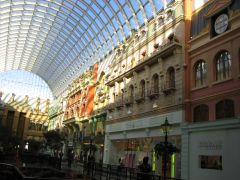
\includegraphics[width=.45\linewidth]{gfx/example_1}} \quad
\subfloat[Pan ma signo.]
{\label{fig:example-b}
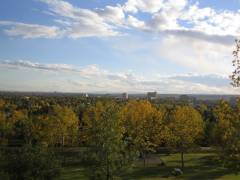
\includegraphics[width=.45\linewidth]{gfx/example_2}} \\
\subfloat[Methodicamente o uno.]
{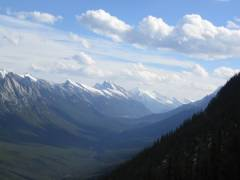
\includegraphics[width=.45\linewidth]{gfx/example_3}} \quad
\subfloat[Titulo debitas.]
{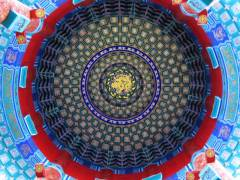
\includegraphics[width=.45\linewidth]{gfx/example_4}}
\caption[Tu duo titulo debitas latente]{Tu duo titulo debitas latente.}\label{fig:example}
\end{figure} % Chapter 2
%% Chapter 3

\chapter{Math Test Chapter} % Chapter title

\label{ch:mathtest} % For referencing the chapter elsewhere, use \autoref{ch:mathtest}

%----------------------------------------------------------------------------------------

\lipsum[13]

%----------------------------------------------------------------------------------------

\section{Some Formulas}

Due to the statistical nature of ionisation energy loss, large fluctuations can occur in the amount of energy deposited by a particle traversing an absorber element\footnote{Examples taken from Walter Schmidt's great gallery: \\ \url{http://home.vrweb.de/~was/mathfonts.html}}.  Continuous processes such as multiple scattering and energy loss play a relevant role in the longitudinal and lateral development of electromagnetic and hadronic showers, and in the case of sampling calorimeters the measured resolution can be significantly affected by such fluctuations in their active layers.  The description of ionisation fluctuations is characterised by the significance parameter $\kappa$, which is proportional to the ratio of mean energy loss to the maximum allowed energy transfer in a single collision with an atomic electron: \graffito{You might get unexpected results using math in chapter or section heads. Consider the \texttt{pdfspacing} option.}
\begin{equation}
\kappa =\frac{\xi}{E_{\mathrm{max}}} %\mathbb{ZNR}
\end{equation}
$E_{\mathrm{max}}$ is the maximum transferable energy in a single collision with an atomic electron.
\[E_{\mathrm{max}} =\frac{2 m_{\mathrm{e}} \beta^2\gamma^2 }{1 + 2\gamma m_{\mathrm{e}}/m_{\mathrm{x}} + \left ( m_{\mathrm{e}} /m_{\mathrm{x}}\right)^2}\ ,\]
where $\gamma = E/m_{\mathrm{x}}$, $E$ is energy and $m_{\mathrm{x}}$ the mass of the incident particle, $\beta^2 = 1 - 1/\gamma^2$ and $m_{\mathrm{e}}$ is the electron mass. $\xi$ comes from the Rutherford scattering cross section and is defined as:
\begin{eqnarray*} \xi  = \frac{2\pi z^2 e^4 N_{\mathrm{Av}} Z \rho
\delta x}{m_{\mathrm{e}} \beta^2 c^2 A} =  153.4 \frac{z^2}{\beta^2}
\frac{Z}{A}
\rho \delta x \quad\mathrm{keV},
\end{eqnarray*}
where

\begin{tabular}{ll}
$z$ & charge of the incident particle \\
$N_{\mathrm{Av}}$ & Avogadro's number \\
$Z$ & atomic number of the material \\
$A$ & atomic weight of the material \\
$\rho$ & density \\
$ \delta x$ & thickness of the material \\
\end{tabular}

$\kappa$ measures the contribution of the collisions with energy transfer close to $E_{\mathrm{max}}$.  For a given absorber, $\kappa$ tends towards large values if $\delta x$ is large and/or if $\beta$ is small.  Likewise, $\kappa$ tends towards zero if $\delta x $ is small and/or if $\beta$ approaches $1$.

The value of $\kappa$ distinguishes two regimes which occur in the description of ionisation fluctuations:

\begin{enumerate}
\item A large number of collisions involving the loss of all or most of the incident particle energy during the traversal of an absorber.

As the total energy transfer is composed of a multitude of small energy losses, we can apply the central limit theorem and describe the fluctuations by a Gaussian distribution. This case is applicable to non-relativistic particles and is described by the inequality $\kappa > 10 $ (\ie, when the mean energy loss in the absorber is greater than the maximum energy transfer in a single collision).

\item Particles traversing thin counters and incident electrons under any conditions.

The relevant inequalities and distributions are $ 0.01 < \kappa < 10 $, Vavilov distribution, and $\kappa < 0.01 $, Landau distribution.
\end{enumerate}

%----------------------------------------------------------------------------------------

\section{Various Mathematical Examples}

If $n > 2$, the identity \[t[u_1,\dots,u_n] = t\bigl[t[u_1,\dots,u_{n_1}], t[u_2,\dots,u_n] \bigr]\] defines $t[u_1,\dots,u_n]$ recursively, and it can be shown that the alternative definition \[t[u_1,\dots,u_n] = t\bigl[t[u_1,u_2],\dots,t[u_{n-1},u_n]\bigr]\] gives the same result. % Chapter 3
%% Chapter X

\chapter{Chapter Title} % Chapter title

\label{ch:name} % For referencing the chapter elsewhere, use \autoref{ch:name} 

%----------------------------------------------------------------------------------------

\section{Section Title}

Content

%------------------------------------------------

\subsection{Subsection Title}

Content

%------------------------------------------------

\subsection{Subsection Title}

Content

%----------------------------------------------------------------------------------------

\section{Section Title}

Content % Chapter 4 - empty template

%\cleardoublepage % Empty page before the start of the next part

%----------------------------------------------------------------------------------------
%	THESIS CONTENT - APPENDICES
%----------------------------------------------------------------------------------------

%\appendix

%\part{Appendix} % New part of the thesis for the appendix

%% Appendix A

\chapter{Appendix Test}

%----------------------------------------------------------------------------------------

\lipsum[13-14]

%----------------------------------------------------------------------------------------

\section{Appendix Section Test}
\lipsum[15]

\graffito{More dummy text}
\lipsum[16]

%----------------------------------------------------------------------------------------

\section{Another Appendix Section Test}
\lipsum[17]

\begin{table}
\myfloatalign
\begin{tabularx}{\textwidth}{Xll} \toprule
\tableheadline{labitur bonorum pri no} & \tableheadline{que vista}
& \tableheadline{human} \\ \midrule
fastidii ea ius & germano &  demonstratea \\
suscipit instructior & titulo & personas \\
\midrule
quaestio philosophia & facto & demonstrated \\
\bottomrule
\end{tabularx}
\caption[Autem usu id]{Autem usu id.}
\label{tab:moreexample}
\end{table}

\lipsum[18]

There is also a useless Pascal listing below: \autoref{lst:useless}.

\begin{lstlisting}[float=b,language=Pascal,frame=tb,caption={A floating example (\texttt{listings} manual)},label=lst:useless]
for i:=maxint downto 0 do
begin
{ do nothing }
end;
\end{lstlisting} % Appendix A
%% Appendix X

\chapter{Appendix Title}

%----------------------------------------------------------------------------------------

% Content begins here % Appendix B - empty template

%----------------------------------------------------------------------------------------
%	POST-CONTENT THESIS PAGES
%----------------------------------------------------------------------------------------
\printnoidxglossaries

%\cleardoublepage
% Bibliography

\label{app:bibliography} % Reference the bibliography elsewhere with \autoref{app:bibliography}

\manualmark % Work-around to have small caps also here in the headline
\markboth{\spacedlowsmallcaps{\bibname}}{\spacedlowsmallcaps{\bibname}} % Work-around to have small caps also
%\phantomsection
\refstepcounter{dummy}

\addtocontents{toc}{\protect\vspace{\beforebibskip}} % Place the bibliography slightly below the rest of the document content in the table of contents
\addcontentsline{toc}{chapter}{\tocEntry{\bibname}}

\printbibliography % Bibliography

%\cleardoublepage% Declaration

\refstepcounter{dummy}
\pdfbookmark[0]{Declaration}{declaration} % Bookmark name visible in a PDF viewer

\chapter*{Declaration} % Declaration section text

\thispagestyle{empty}

Put your declaration here.
\bigskip
 
\noindent\textit{\myLocation, \myTime}

\smallskip

\begin{flushright}
\begin{tabular}{m{5cm}}
\\ \hline
\centering\myName \\
\end{tabular}
\end{flushright}
 % Declaration

%\cleardoublepage% Colophon (a brief description of publication or production notes relevant to the edition)

\pagestyle{empty}

\hfill

\vfill

\pdfbookmark[0]{Colophon}{colophon}

\section*{Colophon}

This document was typeset using the typographical look-and-feel \texttt{classicthesis} developed by Andr\'e Miede. The style was inspired by Robert Bringhurst's seminal book on typography ``\emph{The Elements of Typographic Style}''. \texttt{classicthesis} is available for both \LaTeX\ and \mLyX: 

\begin{center}
\url{https://bitbucket.org/amiede/classicthesis/}
\end{center}

\noindent Happy users of \texttt{classicthesis} usually send a real postcard to the author, a collection of postcards received so far is featured here: 

\begin{center}
\url{http://postcards.miede.de/}
\end{center}
 
\bigskip

\noindent\finalVersionString % Colophon

%----------------------------------------------------------------------------------------

\end{document}
